\documentclass{JoITSRstyle}
\usepackage{graphicx}
\usepackage{times}
%\usepackage{epsfig}
%\usepackage{graphicx}
\usepackage{amsmath}
\usepackage{amssymb}
\usepackage{subfigure}
\usepackage{color}
\usepackage%[usenames,dvipsnames]
{xcolor}
%\usepackage{algorithm}
%\usepackage{algorithmic}
\usepackage{authblk}
\usepackage{abstract}
\usepackage{comment}
%\usepackage{wrapfig}
\usepackage[normalem]{ulem}
\usepackage{url}
\renewcommand\Authands{, }



\begin{document}
\title{Detection of Emergency Telephone Indicators in a Tunnel Environment}

\author[1]{Zhipeng Wang}
\author[1]{Matasaka Kagesawa}
\author[1]{Shintaro Ono}
\author[2]{Atsuhiko Banno}
\author[1]{Takeshi Oishi}
\author[1]{ and\\Katsushi Ikeuchi}

\affil[1]{Institute of Industrial Science, The University of Tokyo, Japan \authorcr
Email: \{wangzp,kagesawa,onoshin,oishi,ki\}@cvl.iis.u-tokyo.ac.jp}
\affil[2]{Advanced Industrial Science and Technology, Ibaraki, Japan  \authorcr
Email: atsuhiko.banno@aist.go.jp}
\twocolumn[
\begin{@twocolumnfalse}
\maketitle
{\normalsize
Positioning of vehicles is important for ITS. In a tunnel environment, most positioning solutions based on GPS sensors or ordinary cameras will fail. For positioning we propose a method to detect emergency telephone indicators in a tunnel environment by using infrared cameras. The proposed detection method makes use of both appearance and motion information of the target objects. By optimizing the detecting pipeline, the method works in real time and produced 100\% detection rate and 0\% false alarm rate in one of our experiments. }

\begin{center}
\emph{\textbf{Keywords: }Object detection, Positioning}
\end{center}
\emph{}
\\
\end{@twocolumnfalse}
]



\section{Introduction}
% no \IEEEPARstart




\begin{comment}
{\color{red}For automatic driving, positioning is very important, and current positioning methods in tunnels often have the problem of accumulated errors. These methods usually rely on the initial position at the entrance of a tunnel obtained from a GPS signal, and the continuous recording of automobile status, i.e. speed and direction of the vehicle. It is obvious that the errors will accumulate. If some signs with position information can be detected while going through the tunnel, the problem of accumulated errors can be solved.}
\end{comment}














\begin{figure}
\centering
\subfigure[]{
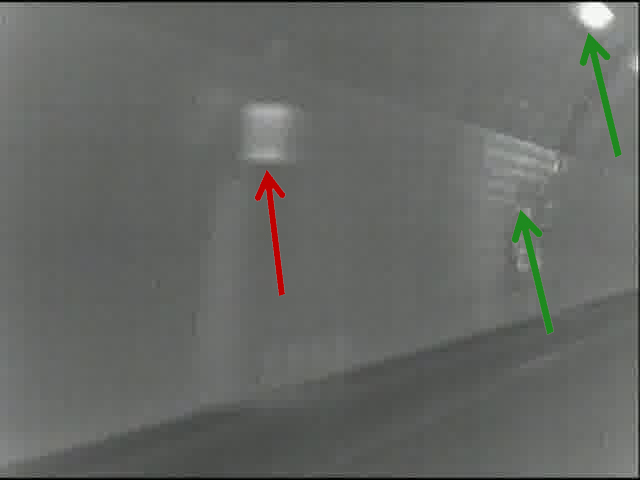
\includegraphics[width=0.22\textwidth,bb=0 0 640 480]{17Orgimg00039.ps}
\label{fig:first:a}}
\subfigure[]{
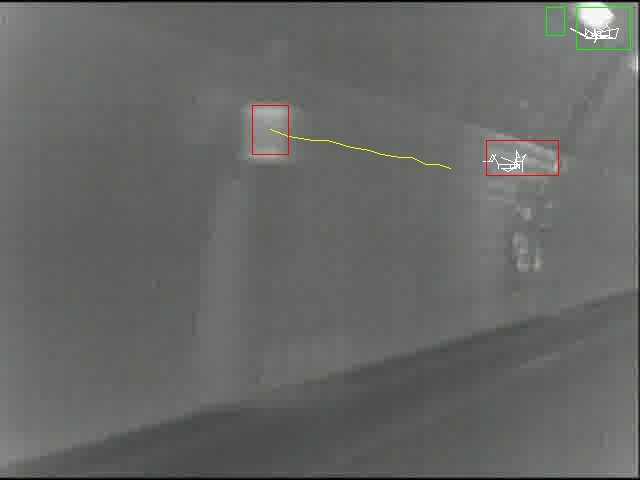
\includegraphics[width=0.22\textwidth,bb=0 0 640 480]{17veriTrjimg00039.ps}
\label{fig:first:b}}
\caption{Original data and detection results. In (a), the red arrow points to the target object: emergency telephone indicator, and the green arrows point to noisy objects. In (b), red rectangles mark detection hypotheses labeled as positive using appearance information, and green rectangles mark negative ones. Yellow trajectories mark detection hypotheses labeled as positive using temporal information, and white trajectories mark negative ones.}
\label{fig:first}
\end{figure}











\section{Related Work}




\section{Emergency Telephone Indicator Detection}
Our proposal can be considered a two-step method. 

\subsection{Keypoint Detection}



let$\{\bf{x}\}$ denote all the sampled points, $I_{\bf{x}}$ the intensity of each point, \begin{comment}$I_{\bf{x}}\sim{\mathcal{N}(\mu_{I_{\bf{x}}},{\sigma_{I_{\bf{x}}}}^2)}$,
\end{comment}
and $l_{\bf{x}}$ the label. If the point is considered as belonging to emergency telephone indicators, $l_{\bf{x}}=1$, otherwise, $l_{\bf{x}}=0$. By setting lower threshold, $I^{th1}_{\bf{x}}$,  and higher threshold, $I^{th2}_{\bf{x}}$, the probability that points belongs to emergency telephone indicators based on their falling into this interval is given by,
\begin{equation}
P(l_{\bf{x}}=1|I^{th1}_{\bf{x}}{\leq}I_x{\leq}{I^{th2}_{\bf{x}}})=
\frac
{P(l_{\bf{x}}=1,I^{th1}_{\bf{x}}{\leq}I_x{\leq}{I^{th2}_{\bf{x}}})} {P(I^{th1}_{\bf{x}}{\leq}I_x{\leq}{I^{th2}_{\bf{x}}})}\;.
\label{eq1}
\end{equation}


\begin{equation}
P(I^{th1}_{\bf{x}}{\leq}I_x{\leq}{I^{th2}_{\bf{x}}}|l_{\bf{x}}=1)=
\frac
{P(l_{\bf{x}}=1,I^{th1}_{\bf{x}}{\leq}I_x{\leq}{I^{th2}_{\bf{x}}})} {P(l_{\bf{x}}=1)}\;.
\label{eq1.1}
\end{equation}


\begin{figure}
\centering
\subfigure[]{
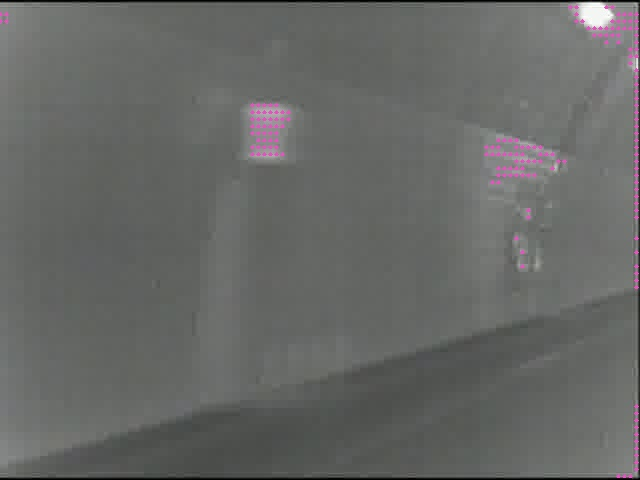
\includegraphics[width=0.22\textwidth,bb=0 0 640 480]{17Kptimg00039.ps}
\label{fig:sec:a}}
\subfigure[]{
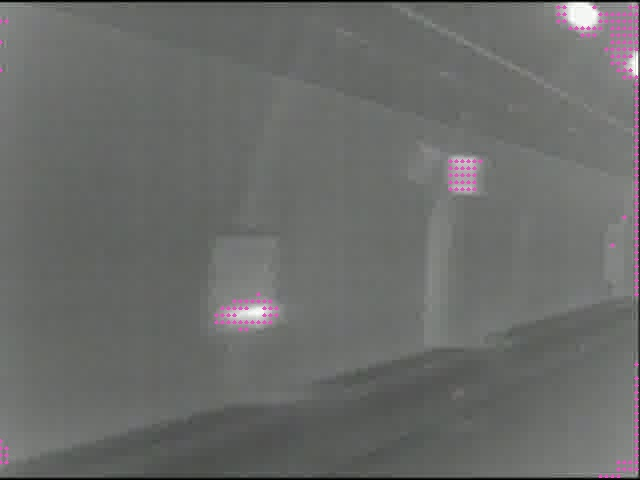
\includegraphics[width=0.22\textwidth,bb=0 0 640 480]{8Kptimg00028.ps}
\label{fig:sec:b}}
\caption{Keypoint detection. }
\label{fig:sec}
\end{figure}
\subsection{Keypoint Verification}


\begin{figure}
\centering
\subfigure[]{
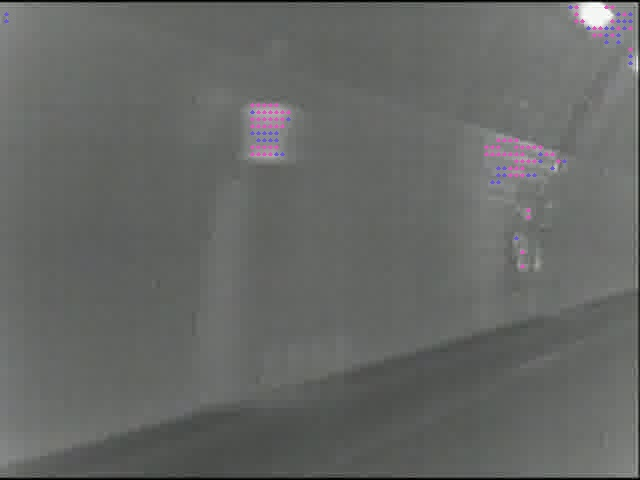
\includegraphics[width=0.22\textwidth,bb=0 0 640 480]{17VeriKptimg00039.ps}
\label{fig:thir:a}}
\subfigure[]{
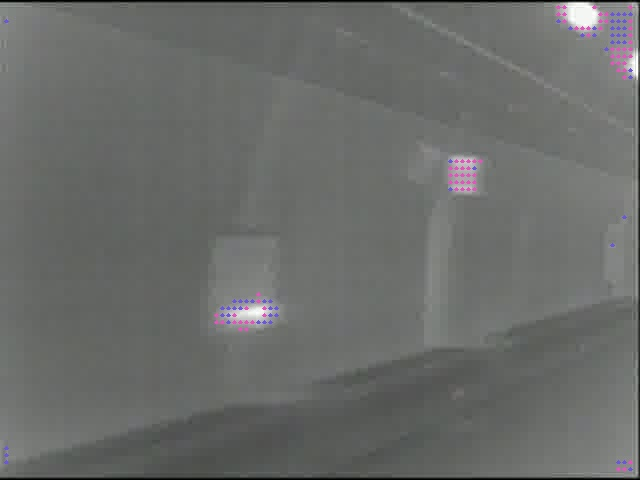
\includegraphics[width=0.22\textwidth,bb=0 0 640 480]{8VeriKptimg00028.ps}
\label{fig:thir:b}}
\subfigure[]{
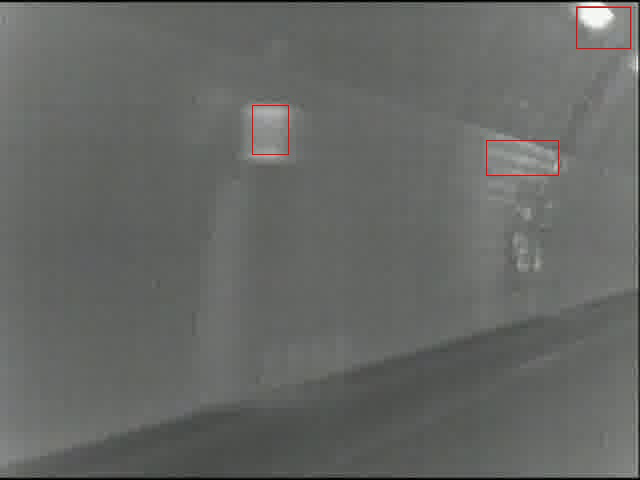
\includegraphics[width=0.22\textwidth,bb=0 0 640 480]{17Rgsimgwl00039.ps}
\label{fig:thir:c}}
\subfigure[]{
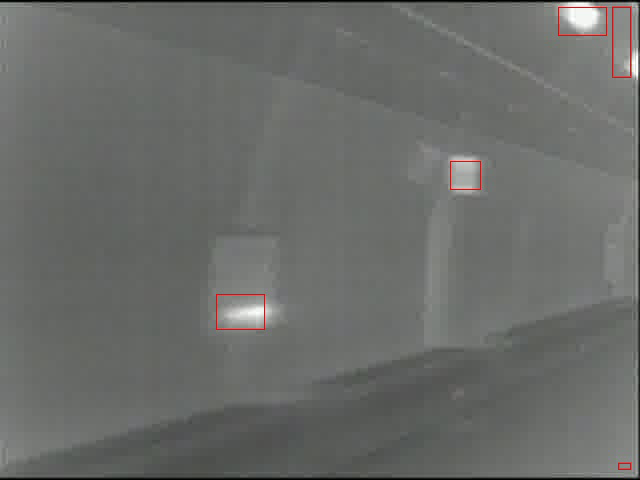
\includegraphics[width=0.22\textwidth,bb=0 0 640 480]{8Rgsimgwl00028.ps}
\label{fig:thir:d}}
\caption{Keypoint verification and clustering. Red circles mark keypoints which pass the verification, while blue marks failed ones. Rectangles mark keypoint clustering results. }
\label{fig:thir}
\end{figure}
\subsection{Keypoint Clustering}



\subsection{Keypoint Cluster Verification by Appearance}

For each keypoint cluster, the smallest bounding rectangle is considered a detection hypothesis, as shown in Figure \ref{fig:thir:c} and Figure \ref{fig:thir:d}. There are three main sources of noise: ordinary lights, other vehicles, and other vehicles' shadows. The global appearance of ordinary lights is different from that of the emergency telephone indicators'. As ordinary lights get further from the infrared camera, the intensities of their corresponding sub-images in the collected data gets lower. At a certain distance, the intensities of the ordinary lights are almost the same as the intensities of the emergency telephone indicators'. For ordinary lights of which the intensities are higher than the intensities of emergency telephone indicators', the transition regions from the lights to tunnel walls will have similar intensities as the emergency telephone indicators'.
This indicates that although locally the emergency telephone indicators share the same appearance with ordinary lights, globally they can still be distinguished by appearance. As for other vehicles and their shadows, their intensity range is very close to the intensity range of the emergency telephone indicators', and they can hardly be distinguished by appearance alone.



At this step, the keypoint clusters are verified by their appearance, ideally excluding keypoint clusters belonging to ordinary lights. An Adaboost machine is trained using intensity histograms of the emergency telephone indicators and ordinary lights. The appearance of other vehicles is close to that of the emergency telephone indicators, and they are not used for training the machine. For training of the machine, labeled 32-dimensional intensity histograms are firstly normalized. Then each weak classifier of the machine makes a decision on one dimension of the intensity histograms. After this step, each keypoint cluster is either labeled as positive or negative.

In this step, to emphasize the Adaboost machine's performance on the positive training examples, we set the initial weights of the positive training examples 7 times as large as the weights of the negative training examples.  Since in practice, whether each keypoint cluster is a target object or not is decided by both appearance and motion information. The difficulties of excluding noisy objects can be left for later steps.
\begin{figure}[b]
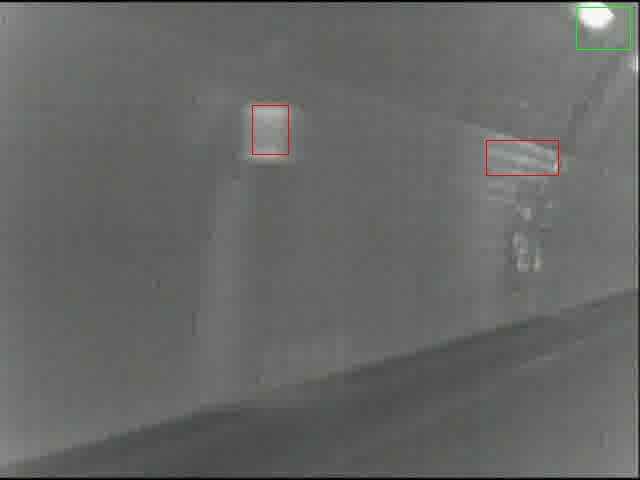
\includegraphics[width=0.22\textwidth,bb=0 0 640 480]{17Rgsimg00039.ps}
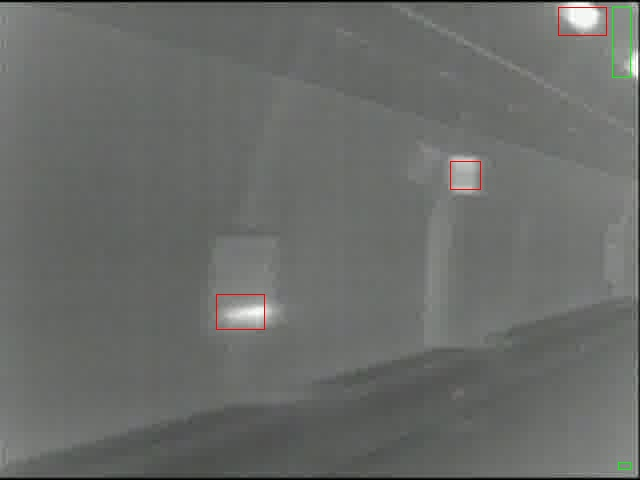
\includegraphics[width=0.22\textwidth,bb=0 0 640 480]{8Rgsimg00028.ps}
\caption{Keypoint cluster verification by appearance. Red rectangles: positive detection hypotheses, and green: negative detection hypotheses.}
\label{fig:fif}
\end{figure}
\subsection{Keypoint Cluster Tracking}

\begin{equation}
\begin{aligned}
{H^*} &= \mathop {\arg \max }\limits_{H \in \eta
} (P(H|\tau,\nu )) \\
&= \mathop {\arg \max }\limits_{H \in \eta }
(\prod\limits_{(T_{\bf{g}}^i,n_{\bf{g}}^j) \in H} {P_{link}(n_{\bf{g}}^j|T_{\bf{g}}^i)} ) \;.
\end{aligned}
\label{eq3}
\end{equation}

\[
\begin{aligned}
&\arg \max\limits_{u_{ij}} \sum\limits_{i = 1}^n \sum\limits_{j = 1}^m u_{ij} \ln P_{link}(n_{\bf{g}}^j|T_{\bf{g}}^i)\\
&
\begin{aligned}
    s.t.:\mbox{ }&u_{ij}=0\mbox{ or }u_{ij}=1,\forall\;i,\forall\;j;\\
    &\sum\limits_{i = 1}^n {u_{ij}} \leq 1\;; \sum\limits_{j = 1}^m {u_{ij}}\leq 1\;.
\end{aligned}
\end{aligned}
\]


\subsection{Keypoint Cluster Verification by Motion}

\begin{equation}
r =| \frac{{\sum\limits_i {\left( {{x^i_{\bf{g}}} -  {\bar x_{\bf{g}}}} \right)\left( {{y^i_{\bf{g}}} -  {\bar y_{\bf{g}}}} \right)} }}{{{{\left[ {\sum\limits_i {{{\left( {{x^i_{\bf{g}}} -  {\bar x_{\bf{g}}}} \right)}^2} \cdot \sum\limits_i {{{\left( {{y^i_{\bf{g}}} -  {\bar y_{\bf{g}}}} \right)}^2}} } } \right]}^{1/2}}}}|\;.
\label{eq4}
\end{equation}

\subsection{Object Detection}







\section{Experimental Results}
We evaluate our method 

\textbf{Data}   7,000 frames are collected for each tour. The frame size is $640\times 480$, the intensity range is [0,255], and the frame rate is 30 frames per second.

\textbf{Implementation Settings} All models are trained using data from the same tour, while evaluated using data from another tour.

To set intensity thresholds for keypoint detection, Gaussian distribution is assumed for the points belonging to emergency telephone indicators. 

About 30,000 intensity histograms of the positive keypoints are sampled, and about 3,000,000 of the negative. When using of $k$-means for clustering the positive intensity histograms, $k$ is set to 40; it is set to 400 for the negative. By using these $k$ values,  both feature sets are over-segmented. 
For keypoint clustering, the threshold to split the mst is set to 40, which is half the largest height of the emergency telephone indicators.




\begin{figure}
{
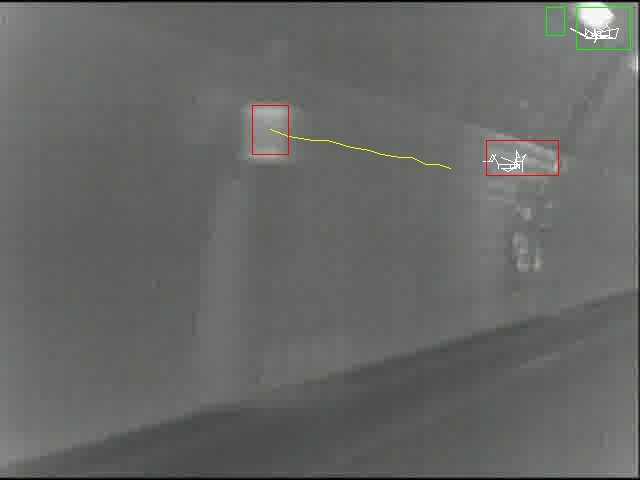
\includegraphics[width=0.22\textwidth,bb=0 0 640 480]{17veriTrjimg00039.ps}
}
{
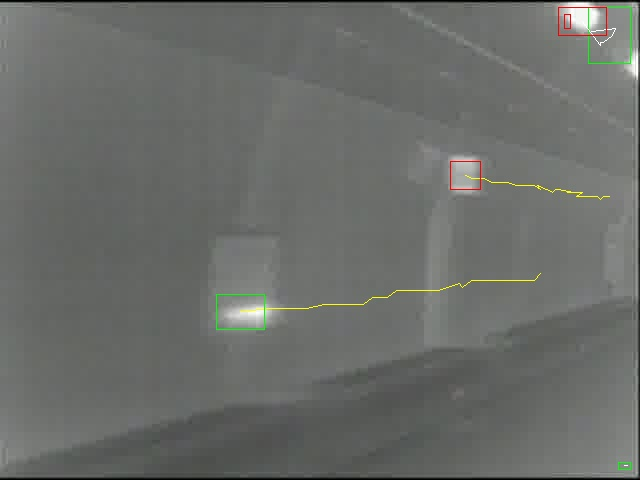
\includegraphics[width=0.22\textwidth,bb=0 0 640 480]{8veriTrjimg00028.ps}
}\\
{
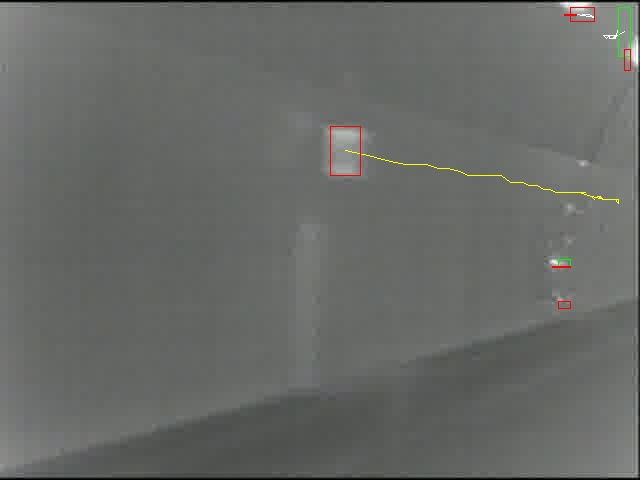
\includegraphics[width=0.22\textwidth,bb=0 0 640 480]{19veriTrjimg00041.ps}
}
{
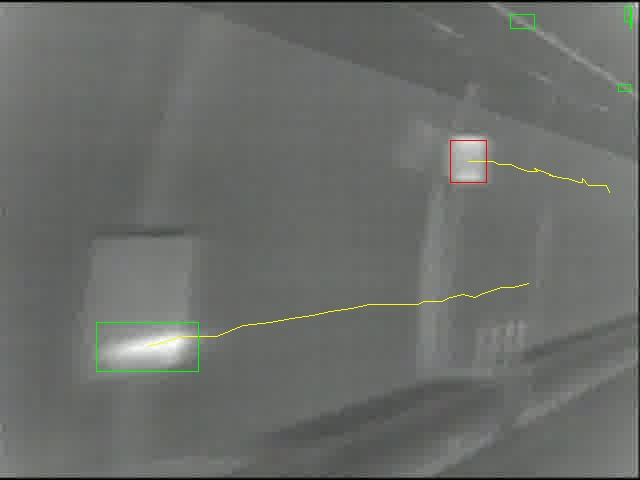
\includegraphics[width=0.22\textwidth,bb=0 0 640 480]{3veriTrjimg00023.ps}
}
\caption{Detection results.}
\label{fig:sixs}
\end{figure}

\textbf{Detection Results}

Using an ordinary desktop computer with Intel Core2 Quad 2.6GHz processors, the method deals with real data at a frame rate of 41 frames per second, and this fulfills real-time requirements.


The detection rate and false alarm rate are evaluated on the keypoint clusters as shown in TABLE \ref{tb:tb2}.
More detection results are shown in Figure \ref{fig:sixs}.
\begin{table}[h]
\centering
\begin{tabular}{lll}
     \hline
     \hline
    total number &	472 + 3304  \\
    correctly labeled &	468   \\
    miss detections &	4 &	  \\
    false alarms &	22    \\
    detection rate &	99.2\% &	  \\
    false alarm rate &	0.7\% &	   \\
   \hline
\end{tabular}
\caption{Detection rate and false alarm rate.}\label{tb:tb2}
\end{table}

While evaluated on a much smaller dataset, the detection rate and false alarm rate of~\cite{wang1} are 90\% and 19\% respectively. Our experiment outperforms~\cite{wang1}, because our sensed images are much clearer, and also because of our more effective training of the Adaboost machine.

The results on the trajectories of decisions are also evaluated. The method correctly detects all of the 22 emergency telephone indicators with no false alarms. The detection rate is 100\%, and the false alarm rate is 0\%.

\section{Conclusion}
We propose an object detection method to detect emergency telephone indicators in a tunnel environment. The method makes use of appearance and motion information of the target objects in a hierarchical manner. With careful optimization of the detection pipeline, the method gives promising results in real time. Based on the detection results, a positioning system in a tunnel environment can be expected.


% conference papers do not normally have an appendix


% use section* for acknowledgement
\section*{Acknowledgment}


The work is in part supported by NEDO. The first author is sponsored by China Scholarship Council. The authors thank Patricia Knapp and Kent Fujiwara for revising suggestions on the manuscript.




{\small
\bibliographystyle{ieee}
\bibliography{egbib}
}









\end{document}
